\documentclass[unknownkeysallowed, 10pt]{beamer}
%\setbeamerfont{structure}{family=\rmfamily} 
\usepackage[utf8]{inputenc} %%
\usepackage[T1]{fontenc}
%\usepackage[french]{babel}
\usepackage{amsthm}
\usepackage{graphicx}
\usepackage{graphics}
\usepackage{hyperref}
\usepackage{multirow} 
\usepackage{tabularx}
\usepackage{longtable}
\usepackage{amsmath}
\usepackage{amsfonts}
\usepackage{amssymb}
\usepackage{booktabs}
\usepackage{caption}
\usepackage{epstopdf}
\usepackage{float}
\usepackage{rotating}
\usepackage{appendixnumberbeamer}
\usepackage{setspace}
\usepackage{verbatim}
\usepackage{tikz}
\usepackage{marvosym}
\usepackage{subcaption}
\usepackage{pifont} %ding symbol
%\usepackage{pgfplots}
%\usetikzlibrary{arrows,intersections,plotmarks,snakes,backgrounds, decorations.markings,matrix,positioning}

\usepackage{natbib}
\usepackage{bibentry}
\nobibliography*


%
\beamertemplatenavigationsymbolsempty
\setbeamertemplate{blocks}[rounded][shadow=true]
\setbeamertemplate{bibliography item}[text]
\setbeamertemplate{caption}[numbered]
\usetheme{cambridgeUS} 
\usecolortheme{rose} %dolphin, orchid, lily, 
\mode<presentation>
{
	\setbeamercovered{transparent}
	\setbeamertemplate{items}[ball]
	\setbeamertemplate{theorems}[numbered]
	%   \setbeamertemplate{headline}[\useinnertheme{default}]
	%   \setbeamertemplate{footline}[frame number]
}
\setbeamertemplate{headline}{%
	\leavevmode%
	\hbox{%
		\begin{beamercolorbox}[wd=1.1\paperwidth,ht=2.5ex,dp=1.125ex]{palette quaternary}%
		\insertsectionnavigationhorizontal{\paperwidth}{\hspace{5em}}{\hspace{5em}}
		\end{beamercolorbox}%
	}
}
%-------------------------------------------------------------------------
\definecolor{exemple}{gray}{0.92}
\definecolor{greenstata}{rgb}{0,0.5,0}
\definecolor{dullmagenta}{rgb}{0.45,0.1,00} 
\definecolor{darkblue}{rgb}{0,0,0.6}
\definecolor{darkgreen}{rgb}{0,0.6,0}
\definecolor{darkred}{rgb}{0.6,0,0}
\definecolor{cyan}{rgb}{0,255,255}
\definecolor{teal}{rgb}{0.0, 0.55, 0.55}

%-------------------------------------------------------------------------
\setbeamercolor*{block title}{fg=darkblue,
bg= blue!20}
\setbeamercolor*{block body}{fg= black,
bg= blue!15}
\setbeamercolor*{block title example}{fg=darkgreen,
bg= green!20}
\setbeamercolor*{block body example}{fg= black,
bg= green!15}
%-------------------------------------------------------------------------
\newenvironment<>{noblock}[1]{%
  \begin{actionenv}#2%
      \def\insertblocktitle{#1}%
      \par%
      \mode<presentation>{%
        \setbeamercolor{block title}{fg=darkred,bg=red!20}
       \setbeamercolor{block body}{fg=black,bg=red!15}
       \setbeamercolor{itemize item}{fg=red}
       \setbeamertemplate{itemize item}[triangle]
     }%
      \usebeamertemplate{block begin}}
    {\par\usebeamertemplate{block end}\end{actionenv}
}
%-------------------------------------------------------------------------
\newenvironment<>{problock}[1]{%
  \begin{actionenv}#2%
      \def\insertblocktitle{#1}%
      \par%
      \mode<presentation>{%
        \setbeamercolor{block title}{fg=darkgreen,bg=green!20}
       \setbeamercolor{block body}{fg=black,bg=green!15}
       \setbeamercolor{itemize item}{fg=darkgreen}
       \setbeamertemplate{itemize item}[triangle]
     }%
      \usebeamertemplate{block begin}}
    {\par\usebeamertemplate{block end}\end{actionenv}
}
%-------------------------------------------------------------------------
\newcommand{\bt}[1]{
\texttt{{\color{darkblue}#1}}
}

\newcommand{\btt}[2]{
\texttt{{\color{darkblue}#1} #2}
}

\newcommand{\ct}[2]{
\texttt{{\color{#1}#2}}
}

\newcommand{\ctt}[3]{
\texttt{{\color{#1}#2} #3}
}



%-------------------------------------------------------------------------
\begin{document}
%-------------------------------------------------------------------------
%-------------------------------------------------------------------------
\title[Micro Econometrics]{The Effect of Depression on Obesity: \\an instrumental variable approach}
\author[HEC - UNIL]{Marco Goretti}
	\institute[]{\small HEC - University of Lausanne}
	\date[May 24, 2016]{ May 24, 2016}


%--------------------------------------------------------------------------
%-------------------------------------------------------------------------
\begin{frame}
\titlepage
\end{frame}



%---------------------------------------------------------------------------
\section{Introduction}
%----------------------------------------------------------------------
%----------------------------------------------------------------------
\begin{frame}{BMI}
%\begin{figure}
%\includegraphics[height=0.8\paperheight]{Figures/auction.jpg}
%\end{figure}

\[
\text{BMI} = \frac{\text{weight}}{\text{height}^2}
\]

\begin{itemize}
\item $\text{BMI} < 18.5 \rightarrow$  underweight
\medskip
\item  $\text{BMI} > 25 \rightarrow$ overweight
\medskip
\item  $\text{BMI} > 30 \rightarrow$ obese
\medskip
\item $\text{BMI} > 40 \rightarrow$ morbidly obese
\medskip
\item  Used as a standard way of estimating body fat percentage which would be a way better metric since it corrects for muscle mass but is long and expensive to measure
\end{itemize}

\end{frame}
%----------------------------------------------------------------------
%----------------------------------------------------------------------

\begin{frame}{Depression score}


\begin{itemize}
\item CESD score: Center for Epidemiologic Studies Depression Scale 
\medskip
\item  Ask 6 negative and 2 positive questions 
\medskip
\item  1 point for every "depressed" answer
	\begin{itemize}
		\item Do you feel depressed? (Yes $\rightarrow 1$ , No $\rightarrow 0$)
		\item  Are you happy? (Yes $\rightarrow 0$ , No $\rightarrow 1$)
	\end{itemize}
\medskip
\item The sum of those points yields a score going from 0 (not depressed) to 8 (severely depressed).
\end{itemize}

\end{frame}
%----------------------------------------------------------------------
%----------------------------------------------------------------------

%----------------------------------------------------------------------
\section{State of the Literature}
%----------------------------------------------------------------------
%----------------------------------------------------------------------
\begin{frame}{\secname}
\begin{block}{}
\bibentry{dave}
\end{block}
\begin{itemize}
\item Seven percentage points increase in the probability of being overweight or obese in women with current or past depression diagnosis (no significant effect in men)
\item This causality is linked to an increase of the economic burden of depression by about 10\% (9.7 billion \$)
\end{itemize}

\begin{block}{}
\bibentry{silver}
\end{block}
\begin{itemize}
\item Somatic symptoms of depression were much higher among women
\end{itemize}
\end{frame}
%---------------------------------------------------------------------------

\section{Data}

\begin{frame}{}
\begin{figure}
	\includegraphics[height=0.8\paperheight]{../proj/fig/obesity.eps}
\end{figure}
\end{frame}

%----------------------------------------------------------------------

\begin{frame}{}
\begin{figure}
	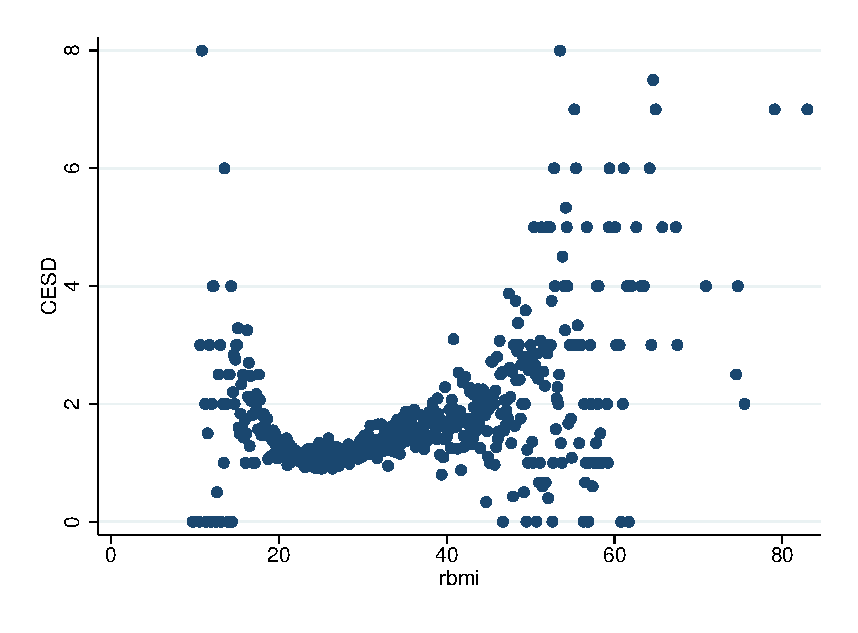
\includegraphics[height=0.8\paperheight]{../proj/fig/cesd.eps}
\end{figure}
\end{frame}

%----------------------------------------------------------------------

\begin{frame}{\secname}

\begin{table}[H]

\begin{center}
\begin{tabular} {@{} l r r r r @{}} \\ \hline
\textbf{    } & \textbf{     CESD} & \textbf{      Male} & \textbf{   Age} & \textbf{   Smoken} \\
\hline
    mean  &   1.210755 &   .5000994 &   64.44591 &    .142326 \\
\hline
\end{tabular}

\end{center}
\end{table}


\begin{table}[H]

\begin{center}

\begin{tabular} {@{} l r r r @{}} \\ \hline
\textbf{   Gender } & \textbf{     CESD} & \textbf{      BMI} & \textbf{     Obese} \\
\hline
       Female  &   1.361464 &   27.53602 &   .2754623 \\
       Male &   1.060107 &   27.90135 &   .2673226 \\
   Total  &   1.210755 &   27.71872 &   .2713917 \\
\hline
\end{tabular}

\end{center}
\end{table}

\end{frame}
%---------------------------------------------------------------------------



%----------------------------------------------------------------------
\section{Model}
%----------------------------------------------------------------------
\begin{frame}{\secname}

\[
\text{Obese} = \beta_0 + \beta_1 \cdot \text{CESD} + \beta_2  \cdot \text{Male} + \beta_3 \cdot \text{Male} \cdot  \text{CESD}+ \beta_4 \cdot \text{Smoked}  
\] \[
+ \beta_5 \cdot \text{Male} \cdot \text{Smoked} +  \delta \cdot \text{wave}  + \xi \cdot \chi + \epsilon
\]

\begin{itemize}
\item  wave is a vector of dummies telling in which wave the observation is  
\item $\xi$ is composed of the controls education level, age and smoking situation of the spouse.
\medskip
\item OLS, ivreg, ivprobit (marginal effects at mean)
\item Depression of the spouse as instrument for own depression
\item Construction of a second instrument for the endogenous interaction Male x CESD
\[
Male \cdot \text{Spouse's CESD}
\]
\end{itemize}


\end{frame}


%----------------------------------------------------------------------
\section{Results}
\begin{frame}{\secname}

\begin{figure}
	\includegraphics[height=0.8\paperheight]{../proj/matlab/1.pdf}
\end{figure}

\end{frame}

\begin{frame}{\secname}
\framesubtitle{scaled}

\begin{figure}
	\includegraphics[height=0.8\paperheight]{../proj/matlab/2.pdf}
\end{figure}

\end{frame}
%---------------------------------------------------------------------------

%----------------------------------------------------------------------
\section{Conclusion}
%----------------------------------------------------------------------
%----------------------------------------------------------------------
\begin{frame}{\secname}
\begin{itemize}
\item Confirmed intuitive result that being depressed increases your BMI
\medskip
\item Effect only weakly significant for males
\medskip
\item Smoking has a very strong effect on being thinner (-16\% probability of being obese)
\medskip
\item Effect increases the cost of depression (\cite{dave})
\end{itemize}


\end{frame}
%---------------------------------------------------------------------------

%----------------------------------------------------------------------
\begin{frame}{}
%\framesubtitle{Table 4}
\begin{center}
{ \LARGE \textbf{Thank you!}} \bigskip

\bigskip
\bigskip
\bigskip
\bigskip



{ \LARGE \textbf{Questions ?}}
\end{center}
\end{frame}
%----------------------------------------------------------------------

\begin{frame}{Bibliography}
\nocite{*}
\bibliographystyle{plainnat}
\bibliography{../paper/bib/bib}
\end{frame}

\appendix
\newcounter{finalframe}
\setcounter{finalframe}{\value{framenumber}}
% Backup frames
\setcounter{framenumber}{\value{finalframe}} 

%----------------------------------------------------------------------
\subsection*{Appendix}
%----------------------------------------------------------------------

\begin{frame}{\subsecname}

\begin{figure}
	\includegraphics[height=0.8\paperheight]{../proj/fig/wavebmi.eps}
\end{figure}

\end{frame}



\begin{frame}{}
\begin{table}[H]
\centering
\resizebox{0.6\textwidth}{!}{\begin{minipage}{\textwidth}%
{
\def\sym#1{\ifmmode^{#1}\else\(^{#1}\)\fi}
\begin{tabular}{l*{3}{c}}
\hline\hline
                    &\multicolumn{1}{c}{(1)}&\multicolumn{1}{c}{(2)}&\multicolumn{1}{c}{(3)}\\
                    &\multicolumn{1}{c}{\shortstack{obese\\reg}}&\multicolumn{1}{c}{\shortstack{obese\\ivreg}}&\multicolumn{1}{c}{\shortstack{obese\\ivprobit marginal}}\\
\hline
CESD depression score&      0.0185\sym{***}&      0.0555\sym{***}&      0.0497\sym{***}\\
                    &   (0.00168)         &   (0.00794)         &   (0.00683)         \\
[1em]
Male x CESD         &    -0.00653\sym{*}  &     -0.0317\sym{**} &     -0.0289\sym{**} \\
                    &   (0.00259)         &    (0.0111)         &    (0.0103)         \\
[1em]
Male                &      0.0336\sym{***}&      0.0688\sym{***}&      0.0636\sym{***}\\
                    &   (0.00781)         &    (0.0145)         &    (0.0137)         \\
[1em]
has smoked          &      -0.150\sym{***}&      -0.166\sym{***}&      -0.167\sym{***}\\
                    &   (0.00995)         &    (0.0106)         &    (0.0113)         \\
[1em]
Spouse has smoked   &      0.0124         &     0.00629         &     0.00580         \\
                    &   (0.00790)         &   (0.00799)         &   (0.00763)         \\
[1em]
Male x has smoked   &      0.0123         &      0.0286\sym{*}  &      0.0301         \\
                    &    (0.0134)         &    (0.0145)         &    (0.0157)         \\
[1em]
Age                 &    -0.00720\sym{***}&    -0.00706\sym{***}&    -0.00687\sym{***}\\
                    &  (0.000497)         &  (0.000498)         &  (0.000479)         \\
[1em]
Spouse's Age        &   -0.000264         &   -0.000291         &   -0.000445         \\
                    &  (0.000493)         &  (0.000495)         &  (0.000473)         \\
\hline
Observations        &      100600         &      100600         &      100600         \\
Education Control   &         Yes         &         Yes         &         Yes         \\
Wave Control        &         Yes         &         Yes         &         Yes         \\
\hline\hline
\multicolumn{4}{l}{\footnotesize \footnotesize Standard errors clustered by id in parentheses}\\
\multicolumn{4}{l}{\footnotesize \footnotesize \sym{*} \(p<0.05\), \sym{**} \(p<0.01\), \sym{***} \(p<0.001\)}\\
\end{tabular}
}

\caption{Regression results over the weight problems dependent variable}
\label{tab:obese}
\end{minipage}}%
\end{table}
\end{frame}

%----------------------------------------------------------------------



\end{document}